\chapter{Desenvolvimento}

\section{Dispositivos utilizados}

\subsection{BeagleBone Black e OSSO Cape}

A BeagleBone Black é uma placa de desenvolvimento \textit{open-source}, desenvolvida pela \textit{Texas Instruments}, do tamanho aproximado de um cartão de crédito. Embora possua um tamanho diminuto, seu hardware é competente o suficiente para permitir rodar distribuições de \textit{Linux} como o Debian (a escolhida para esse projeto).

\begin{figure}[H]
        \begin{center}
                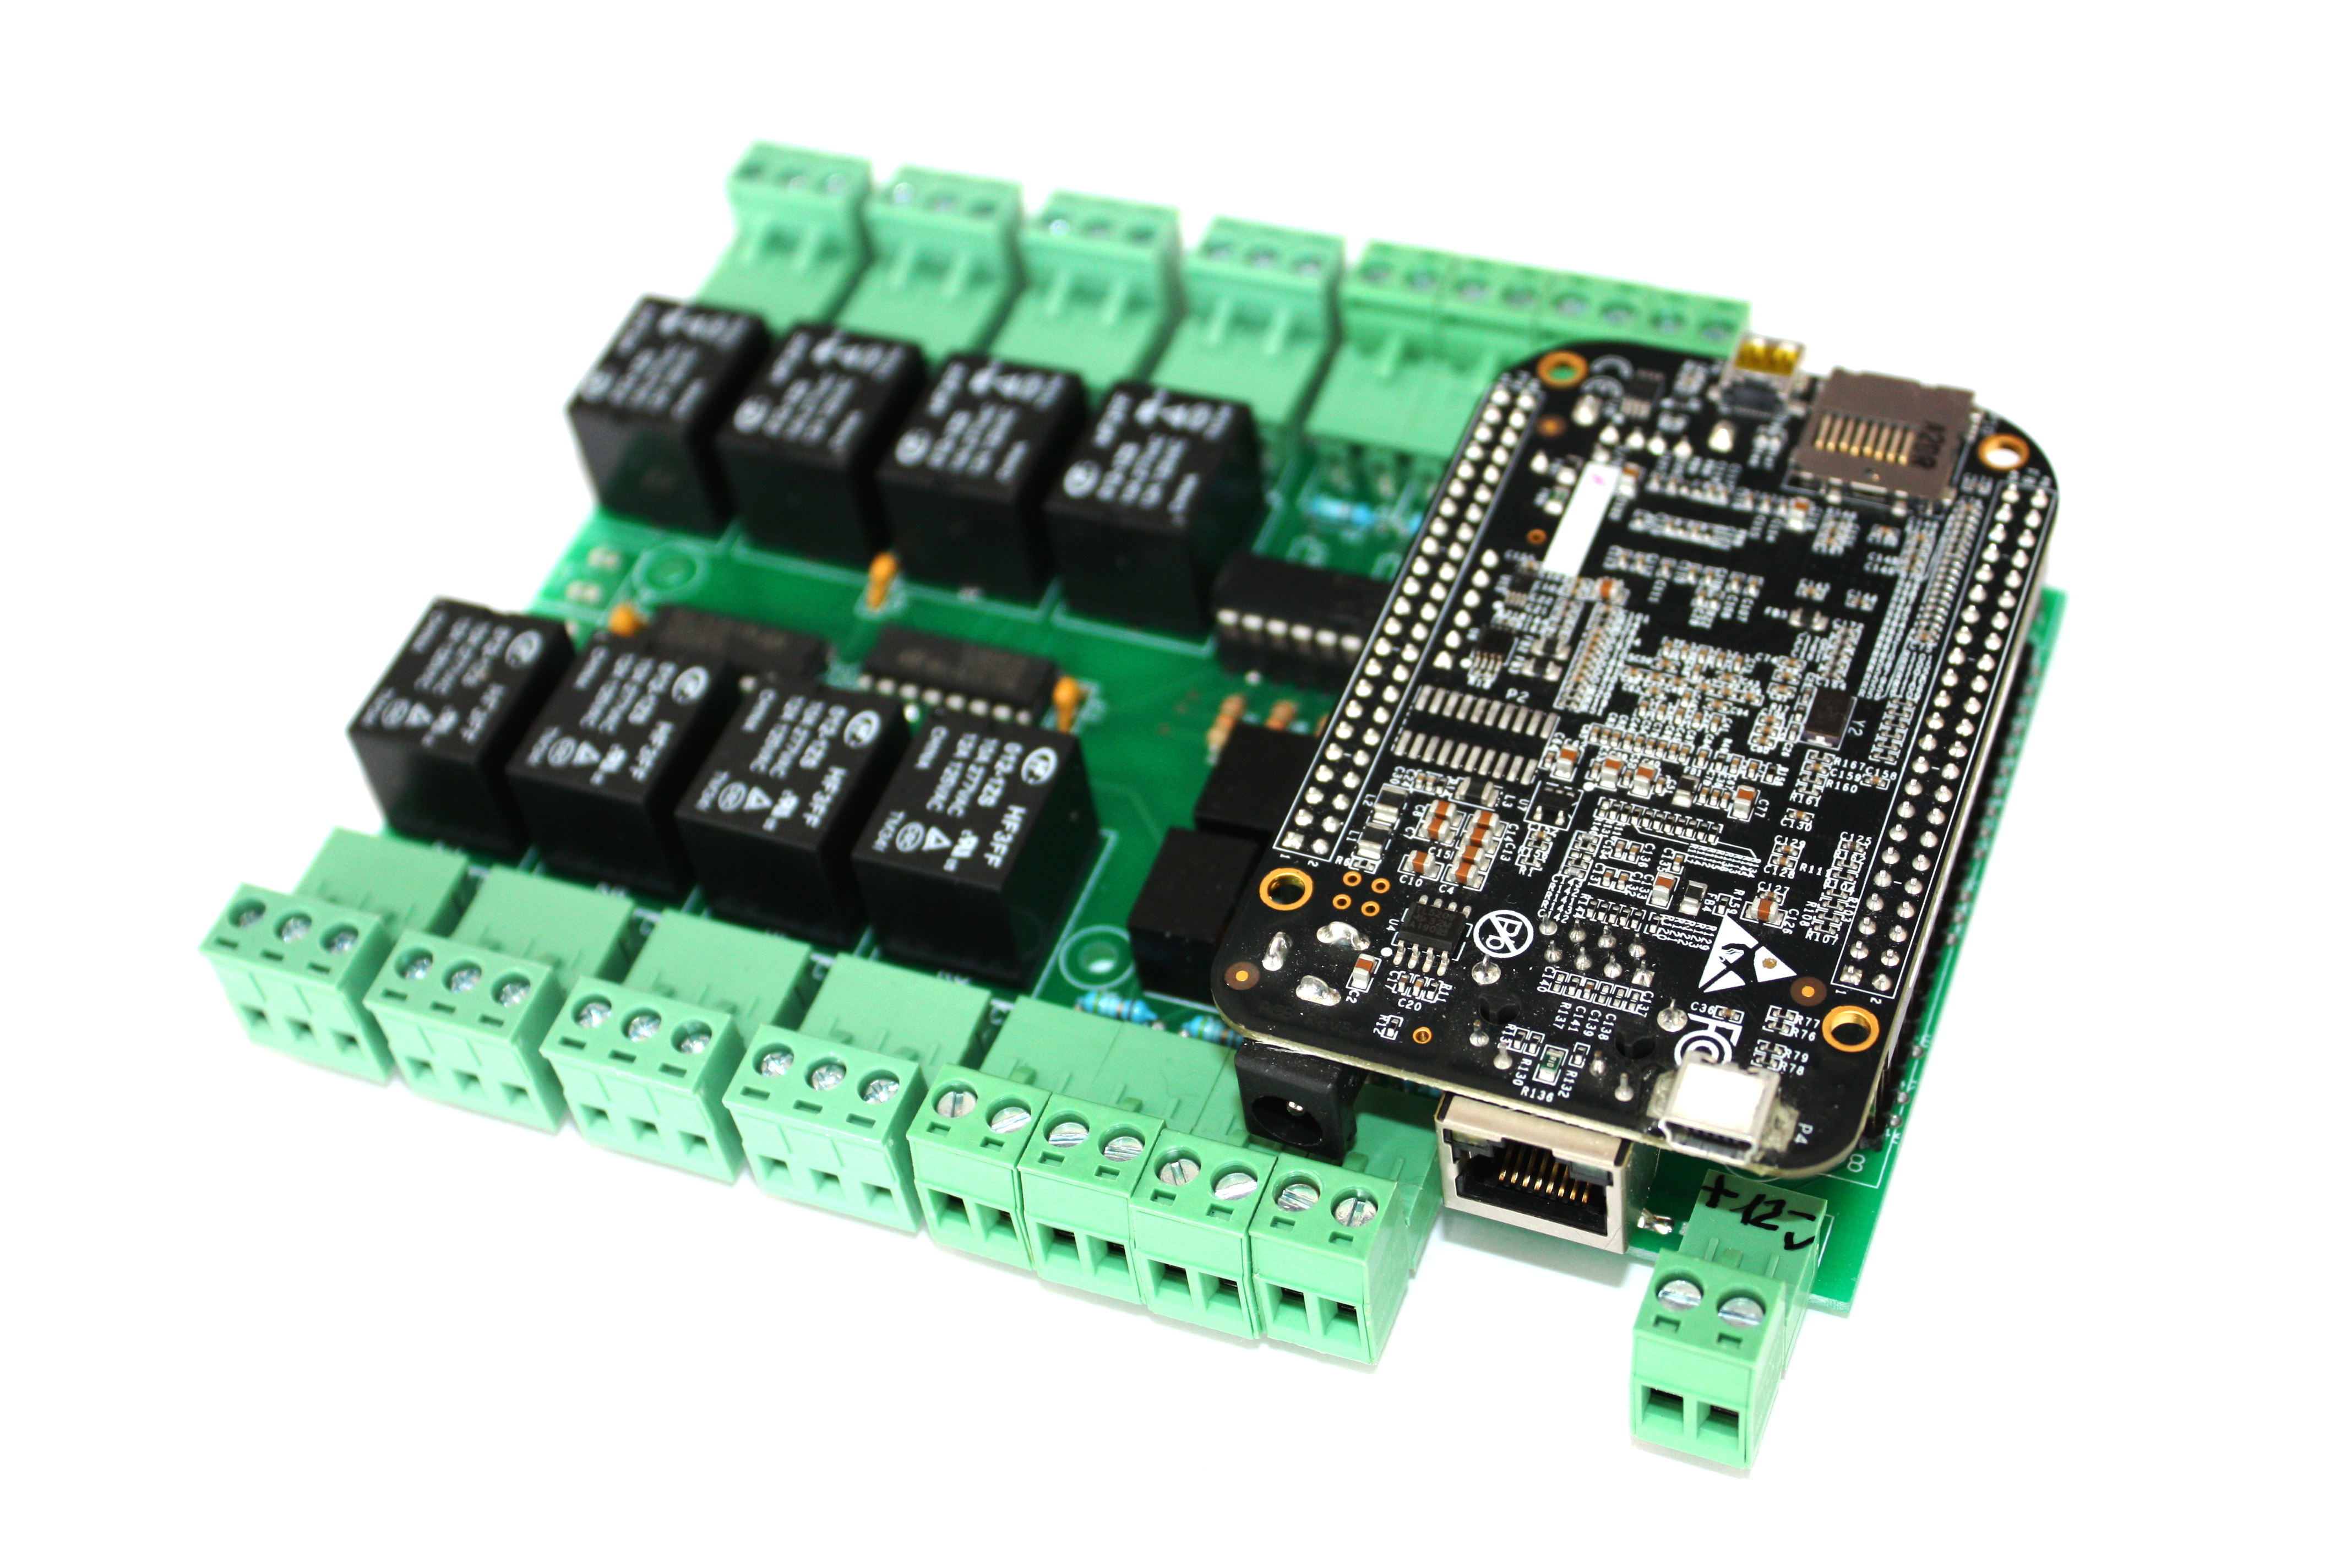
\includegraphics[width=0.75\textwidth,natwidth=585,natheight=180]{assets/images/devices-beaglebone.jpg}
                \caption{BeagleBone Black e OSSO Cape}
                \label{fig:bbb}
        \end{center}
\end{figure}

A BeagleBone permite expansões por meio \textit{capes}, placas não-oficiais que permitem melhor explorar o uso das saídas e entradas. Nesse projeto, foi utilizada a OSSO Cape, sendo que os seguintes recursos facilitaram a implementação do protótipo:

\begin{itemize}
  \item Oito entradas digitais optoacopladas
  \item Oito saídas digitais por meio de relês
  \item Saída RS-485 integrada
  \item Gerenciamento de fontes externas com tensões entre 5 à 24V
\end{itemize}

\subsection{Medidor de Energia Kron Mult-K}

O medidor de energia é essencial para informar tanto ao usuário, quanto ao sistema central, quanta energia foi consumida durante o período do carregamento. O dispositivo escolhido foi o Kron Mult-K, pois esse permite a medição de energia consumida sem a utilização de TCs e os dados são disponibilizados via MODBUS-RTU (conexão RS-485).

\begin{figure}[H]
        \begin{center}
                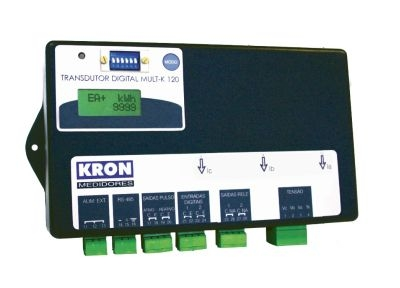
\includegraphics[width=0.75\textwidth,natwidth=400,natheight=288]{assets/images/devices-kron.jpg}
                \caption{Medidor Kron da série Mult-K}
                \label{fig:kron}
        \end{center}
\end{figure}

\subsection{Phoenix EM-CP-PP-ETH Controller}

Os padrões de carregamento rápido utilizam protocolo de comunicação entre carro e estação e, visto a complexidade de decodificar e codificar tais protocolos, foi escolhido utilizar um controlador externo. O Phoenix EM-CP-PP-ETH permite gerenciar carregamentos AC, utilizando três fases em sua alimentação, e realizar todo controle necessário para o sequenciamento de inicialização e finalização de carregamentos.

\subsection{IHM WEG MT}

Para o usuário utilizar a EVSE, é necessária uma interface que apresente as informações necessárias e, além disso, seja robusta a intempéries como calor excessivo e chuva. Para tal, foi escolhida a \ac{IHM} da WEG, linha MT.

Utilizando o \textit{software EasyBuilder 8000}, é possível definir as telas que serão utilizadas pelo usuário, assim como os dados que serão exibidos. Os dados e o controle da IHM são dados por meio de diversos protocolos, dentre eles o MODBUS-TCP, o qual foi escolhido para o projeto.

\begin{figure}[H]
        \begin{center}
                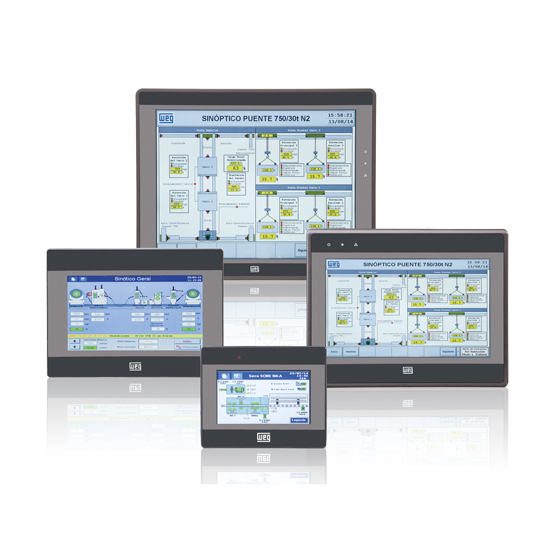
\includegraphics[width=0.75\textwidth,natwidth=400,natheight=288]{assets/images/devices-hmi.jpg}
                \caption{Linha de IHMs MT da WEG}
                \label{fig:ihm}
        \end{center}
\end{figure}

\subsection{Leitor de RFID LotusSmart}

Para iniciar o carregamento na estação, é necessária a utilização de uma \ac{RFID}. É necessária a utilização de um leitor de RFIDs, como o LotusSmart. Ele permite apenas a leitura de cartões de 13.56MHz, visto que há uma variedade de frequências de operação.

O funcionamento de dispositivos como este se dá como se fosse um teclado: ao receber os dados do cartão, o leitor envia seus dados para o computador como se estes fossem digitados pelo usuário. Estes dados são entregues em formato \textit{ASCII}.

\begin{figure}[H]
        \begin{center}
                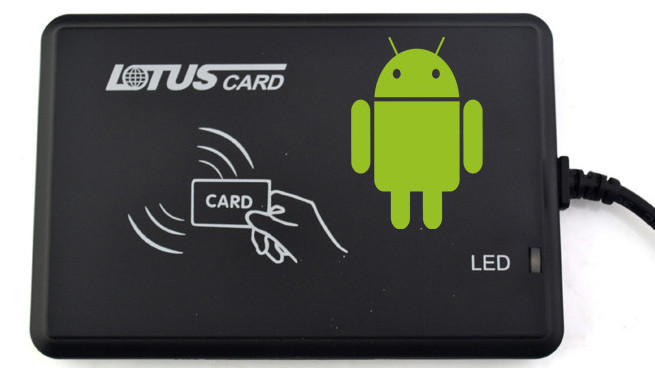
\includegraphics[width=0.75\textwidth,natwidth=655,natheight=368]{assets/images/devices-rfid.jpg}
                \caption{Leitor RFID LotusSmart}
                \label{fig:ihm}
        \end{center}
\end{figure}

\section{Estrutura do Projeto}

A figura \ref{fig:proj-diagram} apresenta o diagrama de conexão dos dispositivos. Como todos os dispositivos são compatíveis com MODBUS, esse foi o protocolo escolhido para a comunicação entre eles. Para a comunicação entre servidor e estação, foi escolhido o protocolo \ac{OCPP}.

A estação possui dois medidores, sendo um de carregamento normal/lento e outro de carregamento rápido. Cada conector possui seu próprio medidores de energia, porém seus controles se dão de forma diferente: o de carregamento rápido utiliza o controlador Phoenix, enquanto o conector normal é controlado pela \textit{BeagleBone} e um relê, visto que ele é somente uma tomada comum e não necessita de nada muito elaborado para inicializar carregamentos (diferente do rápido, onde há um protocolo entre estação e carro).

\begin{figure}[H]
        \begin{center}
                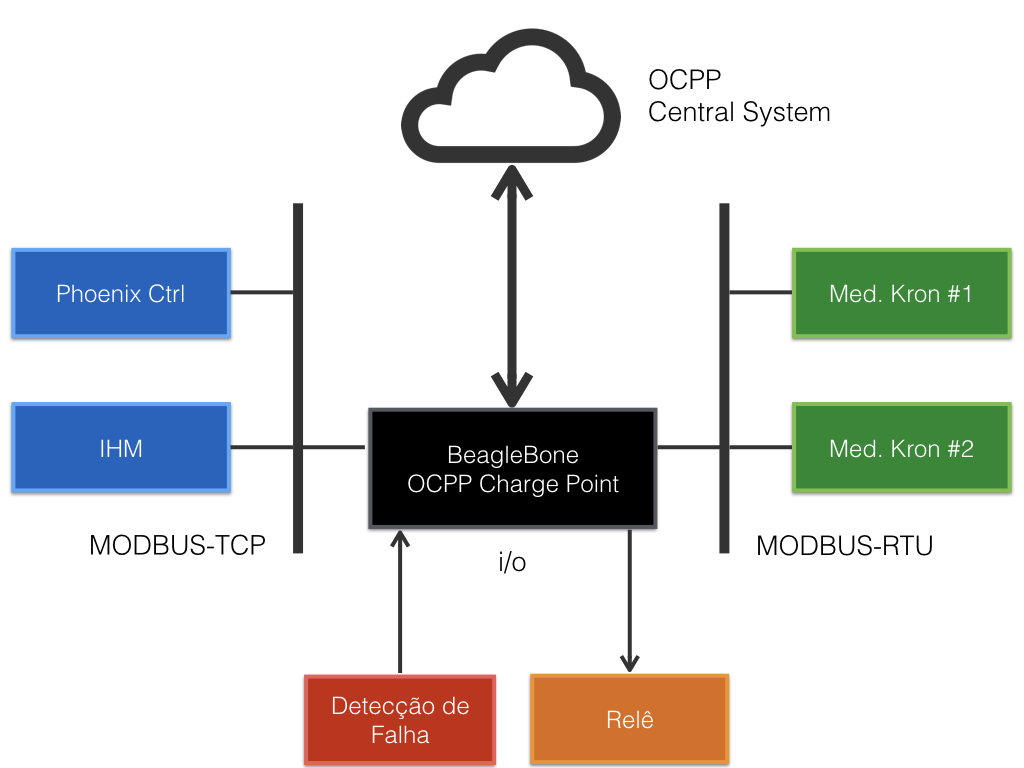
\includegraphics[width=0.8\textwidth,natwidth=400,natheight=288]{assets/images/devices-diagram.png}
                \caption{Diagrama de conexão entre os dispositivos da EVSE}
                \label{fig:proj-diagram}
        \end{center}
\end{figure}

\subsection{Sistema Operacional}

O sistema que roda na BeagleBone é o Debian 8.6 (Jessie) com kernel Linux específico para a \textit{BeagleBone}. Foi instalado o Java 1.7 e houveram modificações em sua device tree para permitir a manipulação das entradas e saídas digitais.

Foram adicionados alguns scripts ao boot do sistema para ativar o acesso à internet e executar o programa logo após a inicialização do sistema.

\subsection{Comunicação entre periféricos}

Visto que todos dispositivos escolhidos suportam MODBUS, esse foi o protocolo escolhido como padrão. A biblioteca \textit{Jamod} foi utilizada para realizar a implementação do protocolo no projeto.

\subsection{Comunicação entre estação e servidores}

A estação implementa o protocolo \ac{OCPP} v1.5, ao qual é suportado por outras estações comerciais vendidas no Brasil, como as da EFACEC, permitindo comunicação com servidores externos. A fundação responsável pelo protocolo disponibiliza um arquivo WSDL, onde é possível criar tanto um servidor quanto um cliente OCPP facilmente.

Para a utilização desse arquivo em Java, foi utilizada a ferramenta wsimport. Ela importa os arquivos e cria classes Java correspondentes a cada \textit{endpoint}. Nem todas funções especificadas pelo protocolo foram implementadas. A tabela \ref{table:ocpp} mostra quais requisições são suportadas.

\begin{table}[]
  \centering
  \caption{Operações OCPP suportadas pela EVSE}
  \label{table:ocpp}
  \begin{tabular}{@{}ll@{}}
    \toprule
    \textbf{Enviada/Recebida} & \textbf{Operação}      \\ \midrule
      Enviada pela Estação      & BootNotification       \\
      Enviada pela Estação      & Heartbeat              \\
      Enviada pela Estação      & StartTransaction       \\
      Enviada pela Estação      & StopTransaction        \\
      Enviada pela Estação      & MeterValues            \\
      Enviada pela Estação      & StatusNotification     \\
      Enviada pela Estação      & Authorize              \\
      Recebida pela Estação     & RemoteStartTransaction \\
      Recebida pela Estação     & RemoteStopTransaction  \\
      Recebida pela Estação     & ChangeConfiguration    \\
      Recebida pela Estação     & GetConfiguration       \\
      Recebida pela Estação     & ChangeAvailability     \\ \bottomrule
    \end{tabular}
\end{table}

\subsection{IHM e do sistema central}

O desenvolvimento da IHM e do sistema central não foi desenvolvido pelo acadêmico, porém são de importância fundamental para o projeto.

\subsection{Software}

O software foi desenvolvido em Java [...]

\section{Testes}

\subsection{Ferramentas de teste}

Para testar a implementação realizada, é necessária uma ferramenta para simular um servidor central. Inicialmente, testou-se a ferramenta \textit{OCPPJS} (http://www.gir.fr/ocppjs/), porém essa apresentou problemas ao lidar com algumas das requisições vindas da EVSE.

Foi criada então uma ferramenta para testes, disponível no Github (https://github.com/brnluiz/ocpp-tools), que implementa parcialmente as funções de um sistema central. Todas operações apresentadas na \ref{table:ocpp} foram implementadas.

Após aberta, a ferramenta ouvirá todas requests das estações que estiverem conectadas à ela e responderá com dados genéricos, possibilitando o funcionamento da estação. Caso o desenvolvedor precise executar alguma requisição às estações, é possível utilizar a \ac{CLI} para tal (os comandos disponíveis são dados pelo manual da ferramenta).

\subsection{Implementações e testes iniciais}

O desenvolvimento inicial se deu no estudo da base de código anterior, que ainda não implementava nada da EVSE funcionalmente, mas possibilitava o teste de cada dispositivo isoladamente. Após esse período inicial, deu-se a implementação do software da estação.

Alguns testes unitários foram desenvolvidos sob o framework de testes \textit{JUnit}, o que permite o programa ser testado antes de ser embarcado na placa de testes. Assim que todos testes passam, o programa é enviado para a \textit{BeagleBone}.

Como as cargas utilizadas durante o teste consumiam pouca energia (fontes AC-DC de dispositivos como notebooks), o medidor de energia teve seu multiplicador de corrente configurado em 100, possibilitando assim simular um consumo alto de forma rápida (sem ter que aguardar várias horas para chegar em 1kWh).

\begin{figure}[H]
        \begin{center}
                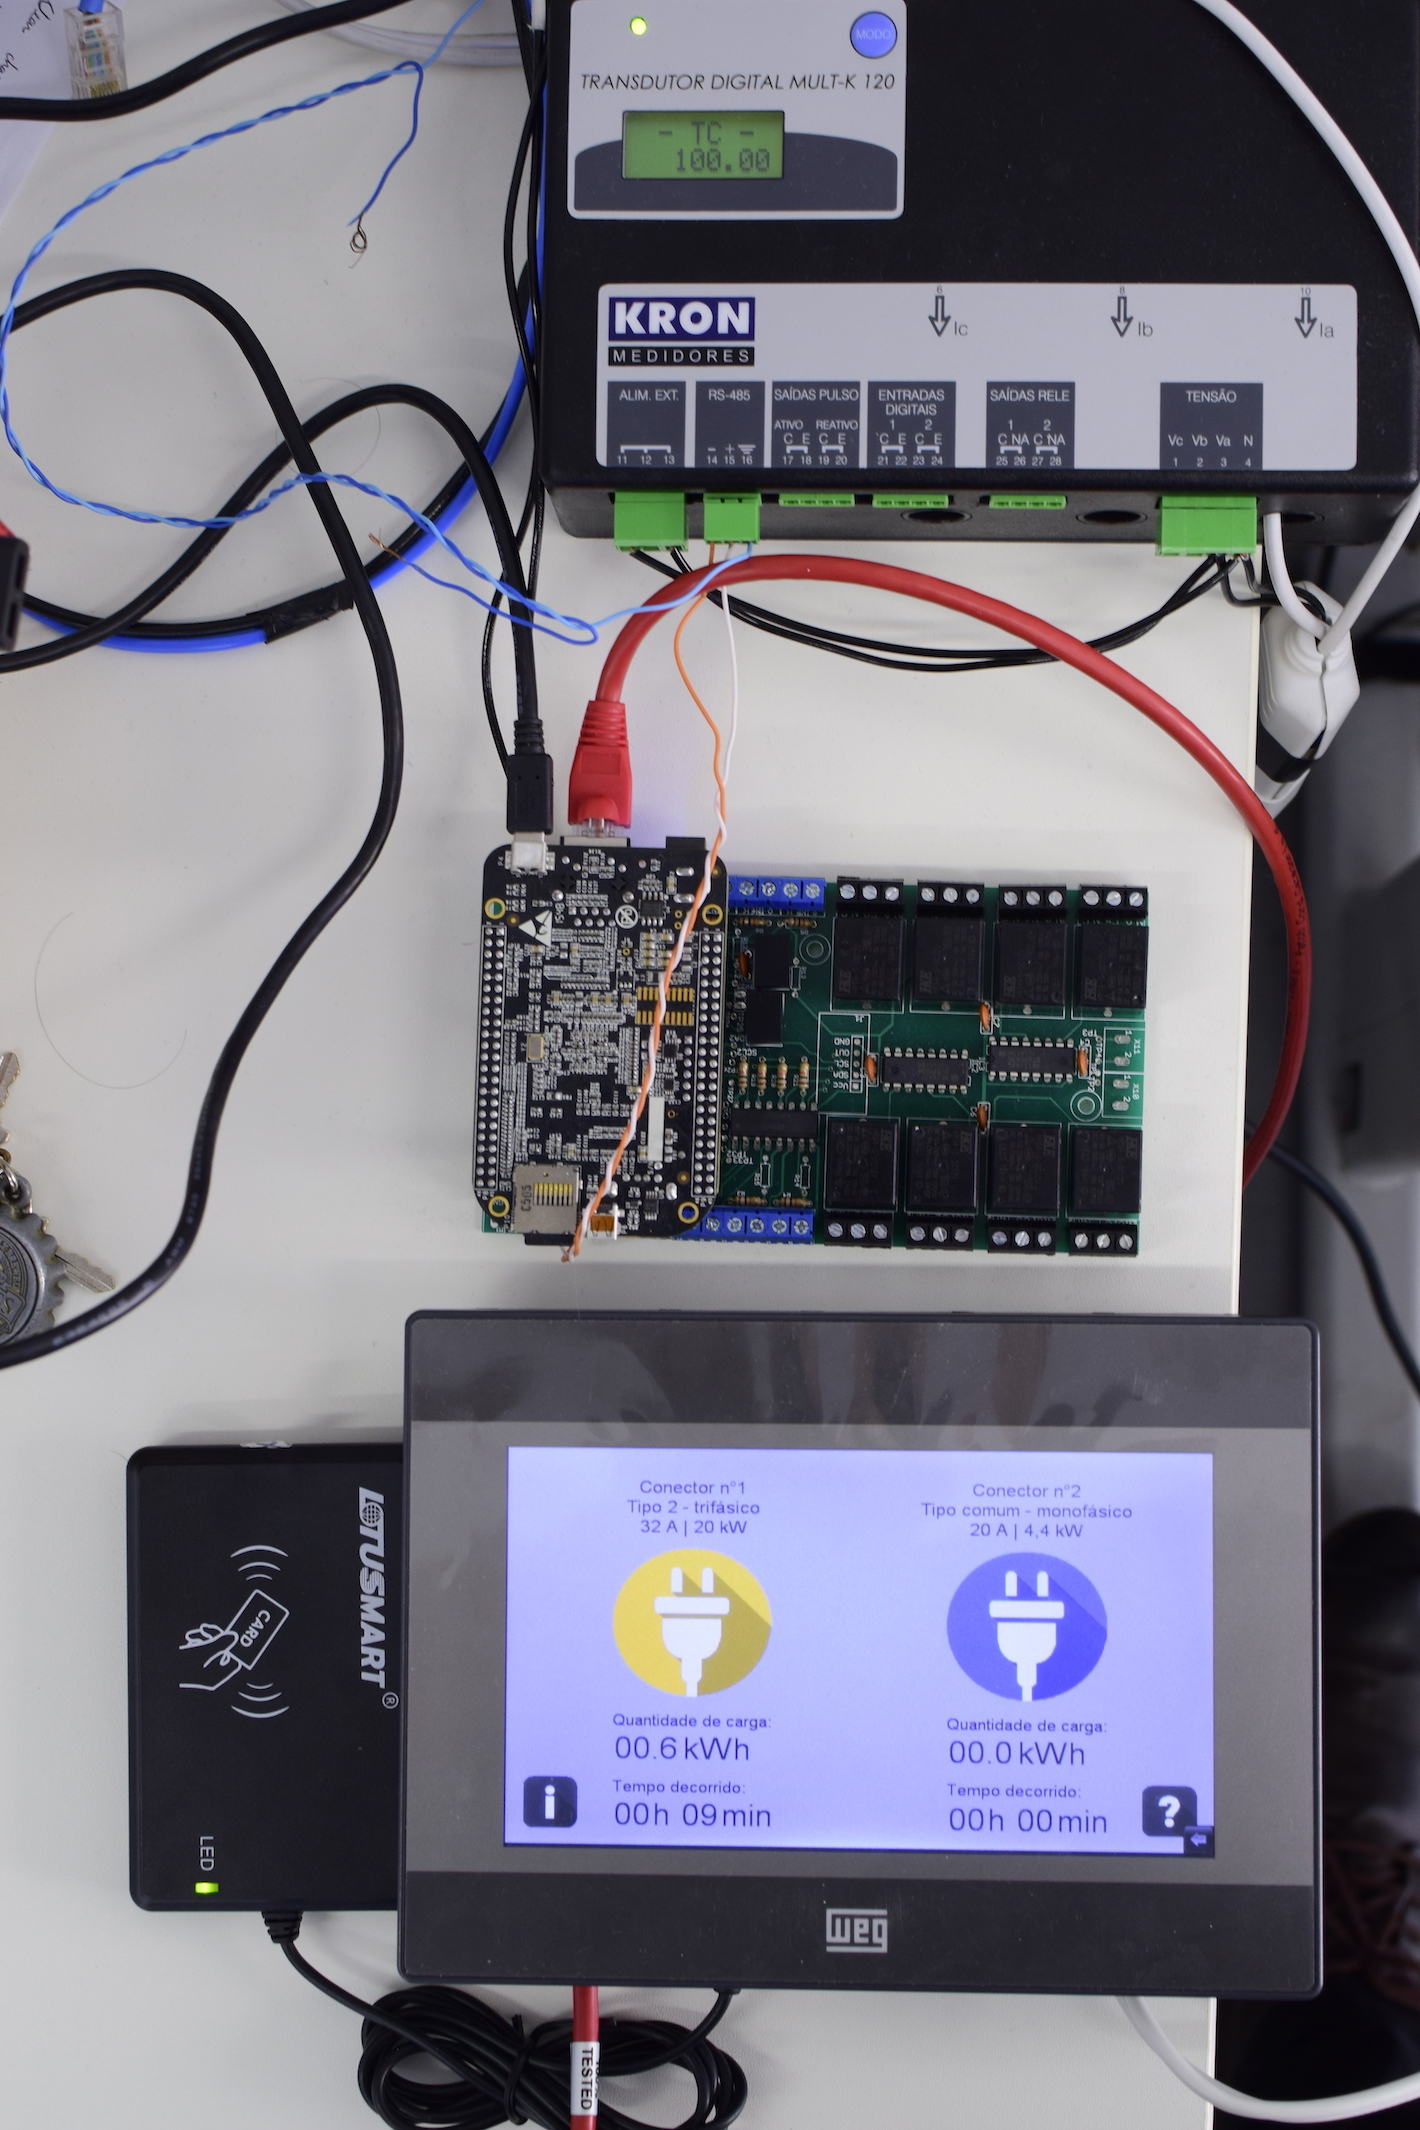
\includegraphics[width=0.6\textwidth,natwidth=2130,natheight=1420,angle=-90]{assets/images/prototype-setup.jpg}
                \caption{Disposição dos dispositivos durante os testes iniciais}
                \label{fig:prototype-setup}
        \end{center}
\end{figure}

\subsection{Testes na estação protótipo}

\begin{figure}[H]
        \begin{center}
                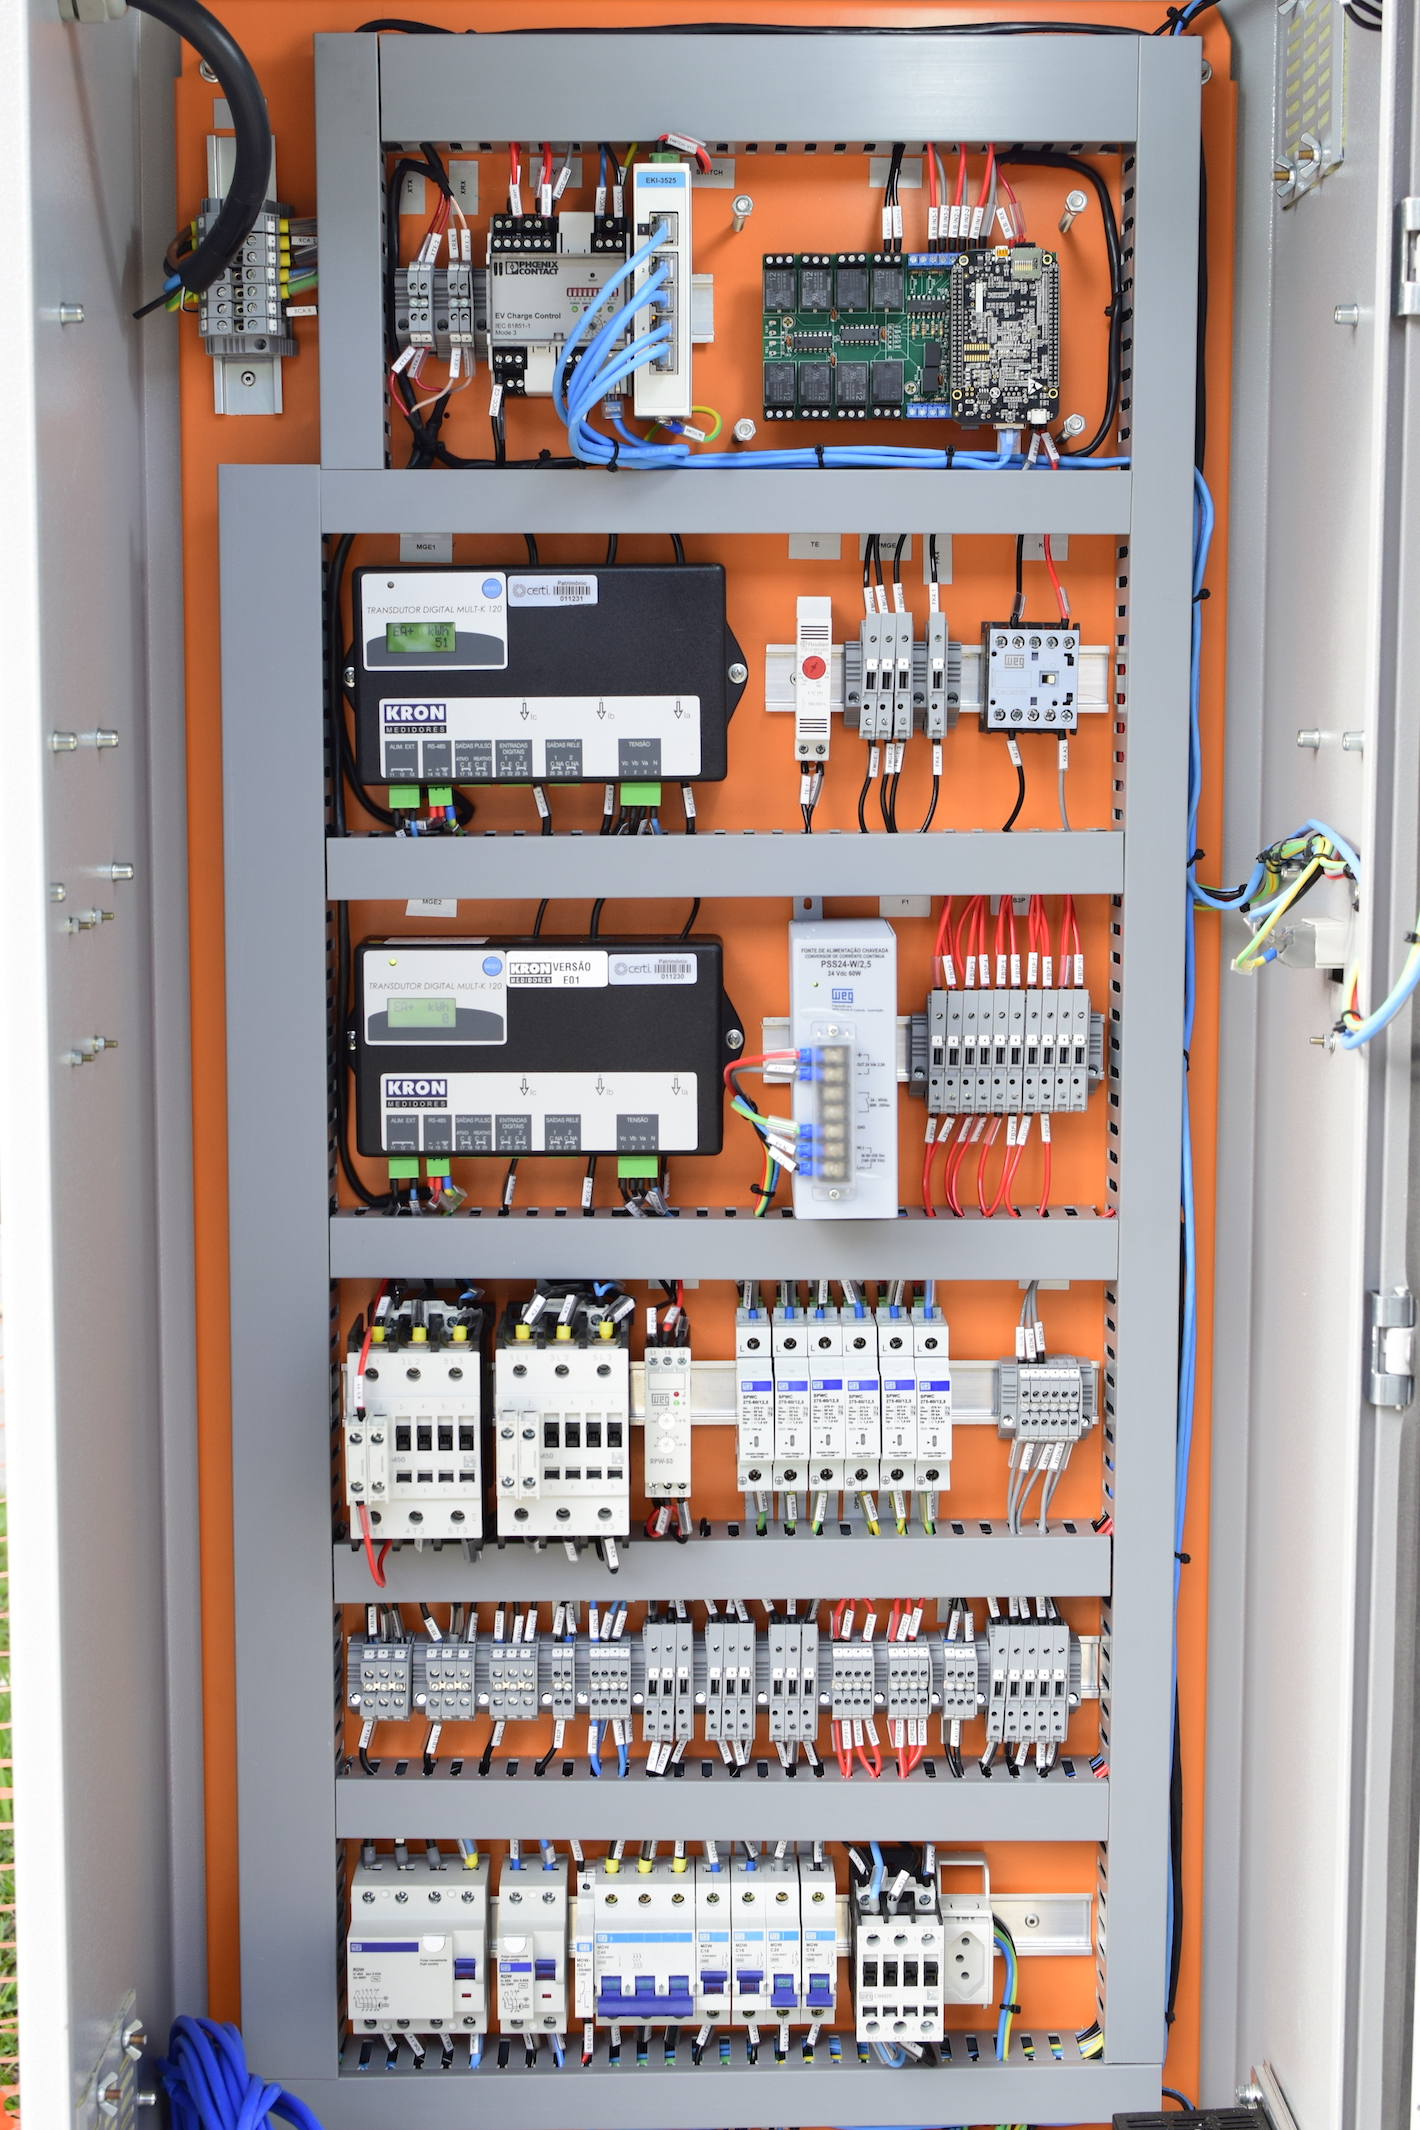
\includegraphics[width=\textwidth,natwidth=1420,natheight=2130]{assets/images/evse-setup.jpg}
                \caption{Disposição dos dispositivos na estação protótipo}
                \label{fig:evse-setup}
        \end{center}
\end{figure}
